\documentclass[crop=false]{standalone}
% --- ПРЕАМБУЛА ДЛЯ ПОДДЕРЖКИ РУССКОГО ЯЗЫКА И МАТЕМАТИКИ ---
\usepackage[T2A]{fontenc}
\usepackage[utf8]{inputenc}
\usepackage[russian]{babel}
\usepackage{amsmath}
\usepackage{geometry}
\usepackage{amssymb}
\usepackage{graphicx}
\usepackage{float}
\usepackage{import}
\geometry{a4paper, top=2cm, bottom=2cm, left=2cm, right=2cm}
\newcommand{\sidecomment}[1]{\marginpar{\raggedright\scriptsize\itshape #1}}
\newcommand{\iu}{\mathrm{i}}

\newcommand{\Def}{%
    \text{Def}%
    \hspace{-0.85em}% Сдвиг назад ровно на середину (подберите под шрифт)
    \raisebox{0.1ex}{/}% Черта
    \hspace{1em}% Возврат к концу слова + небольшой отступ
}

\renewcommand{\Re}{\operatorname{Re}}
\renewcommand{\Im}{\operatorname{Im}}

\ifstandalone
    \newcommand{\lecturebreak}{} % В отдельном файле лекции разрыв не нужен
\else
    \newcommand{\lecturebreak}{\clearpage} % В полной книге - начинаем с новой страницы
\fi

\newcounter{lecturenumber} % Создаем счетчик для нумерации лекций
\newcommand{\lecture}[2]{
    \lecturebreak
    \refstepcounter{lecturenumber} % Увеличиваем счетчик на 1
    \par\vspace{2em}\noindent % Отступ сверху и убираем абзацный отступ
    {\Large\bfseries % Делаем заголовок крупным и жирным
    Лекция \thelecturenumber: #1 % Выводим "Лекция N: Тема"
    \hfill % Растягиваем пробел, чтобы дата была справа
    \large\textit{#2}} % Выводим дату курсивом
    \par\vspace{1em} % Небольшой отступ снизу
    \addcontentsline{toc}{section}{Лекция \thelecturenumber: #1} % Добавляем в оглавление
    \par
}

\newcommand{\TwoCols}[2]{%
  \par\noindent % Начать с новой строки без отступа
  \begin{minipage}[t]{0.48\textwidth}
    #1
  \end{minipage}% <-- Важный '%' для удаления пробела
  \hfill % Растягивающийся пробел между колонками
  \begin{minipage}[t]{0.48\textwidth}
    #2
  \end{minipage}% <-- Важный '%' для удаления пробела
  \par%
}

\pagestyle{plain} % Включаем нумерацию страниц\
\begin{document}
\lecture{}{03.04}
% тебя на этой лекции не было, списано из лекции Дениса
\section{Статические Инварианты}
В контексте твёрдого тела:
\[I_1 = R^2 \qquad I_2 = (\bar M_P, \bar R)\]
\begin{proof}
    \[\bar M_Q = \bar M_P + \bar R \times \overline{PQ} \qquad (\bar M_Q, \bar R) = (\bar M_P, \bar R) + \underbracket{(\bar R \times \overline{PQ} , \bar R)}_0\]
\end{proof}
\Def Динамо — совокупность коллинеарных силы и момента
\[\bar F, \quad \bar M: \qquad \bar F \| \bar M\]

\noindent \keypoint Если $I_1 \cdot I_2 \neq 0$, то произвольную систему сил можно свести к динаме
\begin{proof}
    Докажем, что существует $P^*$:
     \[\bar M_{P^*} = k \bar R\]
     \[\bar M_{P^*} = \bar M_P + \bar R \times \overline{P P^*} = k \bar R\]
     \[I_2 = (\bar M_P , \bar R) =k R^2  = k I_1 \qquad k = \frac{I_2}{I_1}\]
     \[\bar M_P + \bar R \times \overline{P P^*} = \frac{I_2}{I_1} \bar R \qquad \bar R \times \overline{P P^*} = \begin{pmatrix}
        R_x \\ R_y \\ R_z
     \end{pmatrix} \times \begin{pmatrix}
        x - x_P \\ y - y_P \\ z - z_P
     \end{pmatrix}\]
     \[\begin{cases}
        M_{p x} + R_y (z - z_P) - R_z (y - y_P) = \frac{I_2}{I_1} R_x , \\
        M_{p y} - R_x (z - z_P) + R_z (x - x_P) = \frac{I_2}{I_1} R_y , \\
        M_{p z} + R_x (y - y_P) - R_y (x - x_P) = \frac{I_2}{I_1} R_z
     \end{cases}\]
    \end{proof}
\begin{figure}[H] 
    \centering
    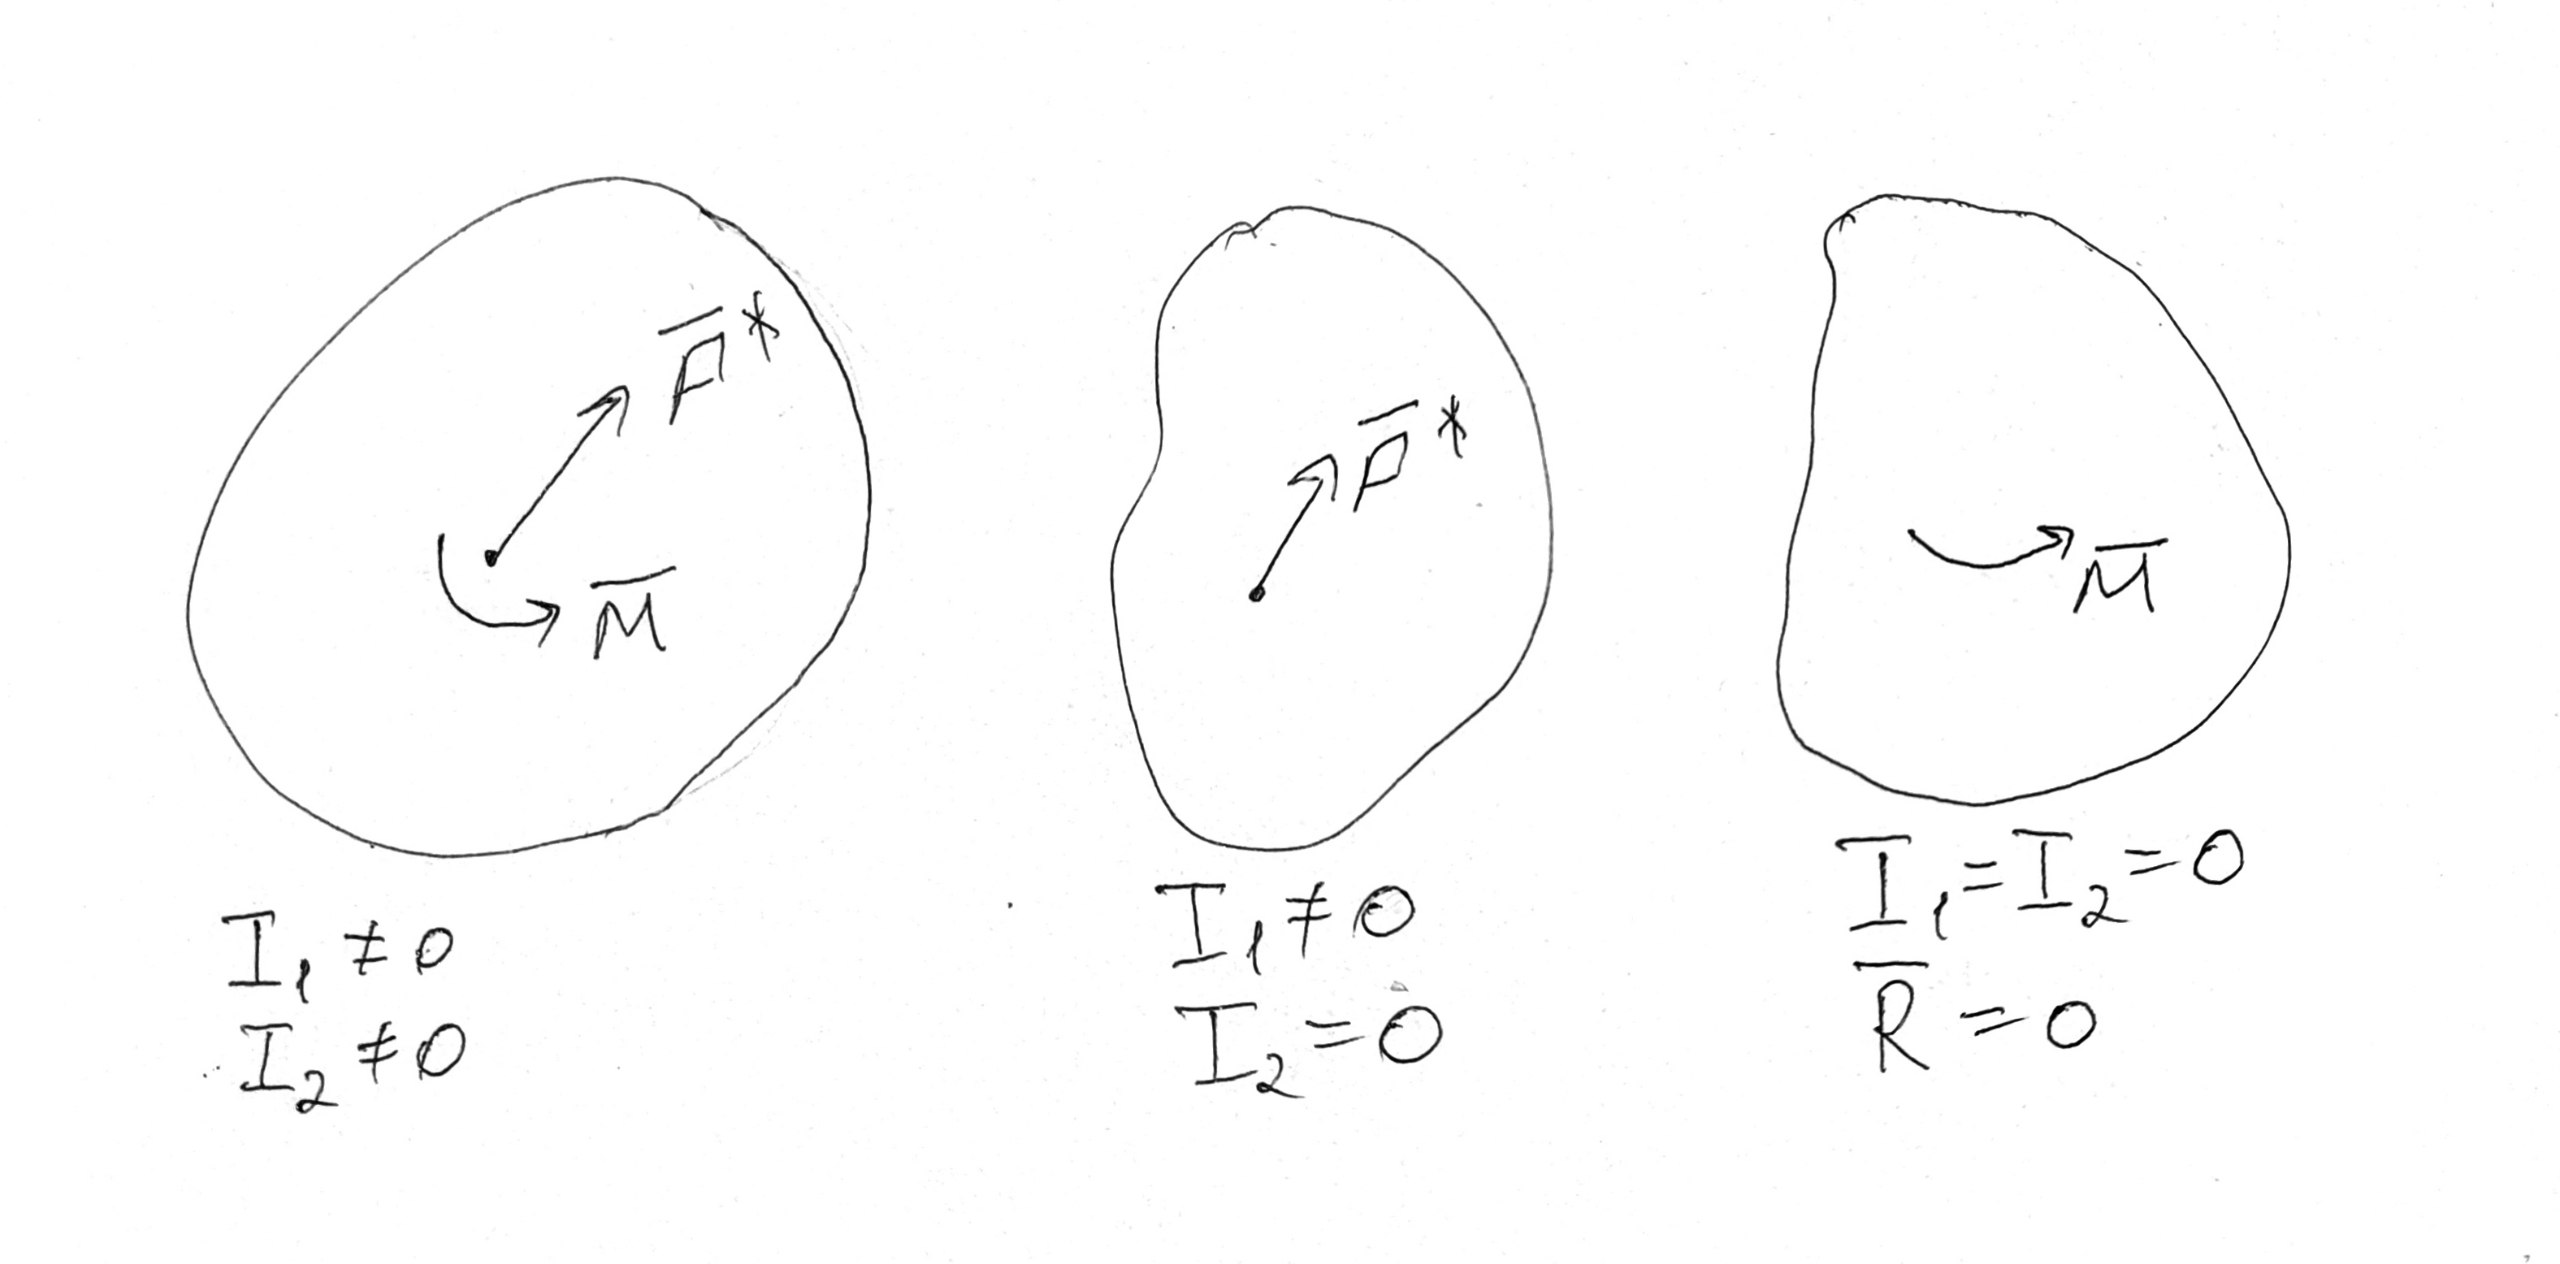
\includegraphics[width=0.5\textwidth]{dinamo.jpg}
    \caption{}
    \label{fig:myimage} 
\end{figure}
    При $I_1 = I_2 = 0$ ось динамы не определена
\section{Основные динамические величины}
\begin{enumerate}
    \item Количество движения системы (импульс)
    \[\bar Q = \sum_{k=1}^{N} m_k \bar v_k\]
    
    \item момент количества движения(кинетический момент)
    \[\bar K_O = \sum_{k=1}^{N} \bar r_k \times m_k \bar v_k \qquad \bar K_P = \sum_{k=1}^{N} (\bar r_k - \bar r_P) \times m_k \bar v_k\]

    \item Кинетическая энергия
    \[T = \frac{1}{2} \sum_{k=1}^{N} m_k v_k^2\]
\end{enumerate}
\Def Центр масс системы — точка
\[\bar r_c = \frac{1}{M} \sum_{k=1}^{N} m_k \bar r_k \qquad M = \sum_{k=1}^{N} m_k\]
Упр: доказать, что если на тело действует только сила тяжести(или другие системы парралельных сил, пропорциональных массе), то равнодействующая будет действовать на центр масс

\noindent \keypoint
\[\dot{\bar r}_C = \bar v_C = \frac{1}{M} \sum_{k=1}^{N} m_k \bar v_K = \frac{1}{M} \bar Q\]


\section{Основные теоремы динамики}
Теоремы об изменении основных динамических величин

для каждой есть дифференциальная и интегральная формулировки

\keypoint
\[\dot{\bar Q} = M \bar w_C = \sum_{k=1}^{N} m_k \dot{\bar v}_k = \sum_{k=1}^{N} m_k w_k = \sum_{k=1}^N F_k = \bar R\]
\[M \bar w_C = \bar R\]
Если $\bar R = 0$, то центр масс либо покоится, либо движется равномерно прямолинейно

Интегральная форма:
\[\Delta \bar Q = \bar Q_2 - \bar Q_1 = \int_{t_1}^{t_2} \bar R dt \quad \text{ — импульс силы }\]

\noindent \keypoint

\[
\begin{aligned}
\dot{\bar K}_P &= \frac{d}{d t}\left(\sum_{k=1}^{N} (\bar r_k - \bar r_P) \times m_k \bar v_k \right)
= \sum_{k=1}^{N} (\dot{\bar r}_k - \dot{\bar r}_P) \times m_k \bar v_k  + \underbracket{\sum_{k=1}^{N} (\bar r_k - \bar r_P) \times \underbracket{m_k \bar w_k}_{\bar F_k}}_{\bar M_P}
\\ &= \sum_{k=1}^N \bar v_k \times m_k \bar v_k - \sum_{k=1}^N \bar v_P \times m_k \bar v_k +\bar M_P = -\bar v_P \times \sum_{k=1}^N m_k \bar v_k + \bar M_P
\\ &= - \bar v_P \times \bar Q + \bar M_P = \bar Q \times v_P + \bar M_P
\end{aligned}
\]
\[\boxed{\dot {\bar K}_P  = \bar Q \times \bar v_P + \bar M_P}\]
Заметим:
\[\bar v_P = 0 \iff \dot {\bar K}_P = \bar M_P \]
Заметим:
\[\bar v_P = \bar v_C \iff \dot{\bar K}_C = \bar M_C\]
\begin{proof}
    \[\bar Q \times \bar v_C = M \bar v_C \times \bar v_C = 0\]
\end{proof}
Интегральная форма:
\[\Delta \bar K_O = \int_{t_1}^{t_2} \bar M_O dt \text{ — импульс момента}\]

\noindent \keypoint
\[\dot T = \frac{1}{2} \frac{d}{d t}\left(\sum_{k=1}^N m_k v_k^2\right) = \sum_{k=1}^N m_k (\dot{\bar v}_k, \bar v_k) = \sum_{k=1}^N (m_k \bar w_k,\bar v_k) = \sum_{k=1}^N (\bar F_k, \bar v_k)\]
это совопупная мощность всех сил и это мощность внутренних и внешних сил

\[d T = \frac{1}{2} \sum_{k=1}^N m_k d v_k^2 = \sum_{k=1}^N m_k (\bar v_k, d \bar v_k) = \sum_{k=1}^N (m_k \bar w_k d t, \bar v_k) = \sum_{k=1}^N (\bar F_k, \bar v_k d t) = \sum_{k=1}^N (\bar F_k , d r_k) = d' A\]
Работа всех сил на действительных перемещениях
\[\boxed{\dot T = \sum_{k=1}^N(\bar F_k, \bar v_k)}\]
\[d T = d' A\]
Интегральная форма:
\[T_2 - T_1 = \int_{t_1}^{t_2} d' A = A_{1 2}\]

\begin{theorem}[Закон сохранения импульса]
Если главный вектор равен 0, 

То кинетический момент сохраняется
\end{theorem}

\begin{theorem}[Законы сохранения момента]
    \begin{itemize}
        \item 
        Если главный момент нуль
        
        То кинетический момент сохраняется
        
        \item
        Если главный момент относительно центра масс нуль
        
        То кинетический момент сохраняется
    \end{itemize}
\end{theorem}
\end{document}